\section{ELECTR}
\label{sELECTR}

\hypertarget{sELECTRhy}{The}
ELECTR\index{ELECTR|textbf} module of NJOY is designed to
produce complete and accurate multigroup electroatomic
\index{electroatomic} cross sections from ENDF/B-IV, -V -VI or
-VII data\cite{HUGO}. It will also work with the newer formats
developed for ENDF/B-VII. ELECTR produces restricted cross
sections\index{restricted cross sections} consistent with a solution
of the multigroup Boltzmann-Fokker-Planck (BFP)
equation. Total, elastic, inelastic (collision and bremss\-trahlung)
cross sections can be averaged using a variety of group
structures\index{group structures} and weighting
functions.\index{weight functions} The Legendre components of the
within-group elastic and group-to-group inelastic collision cross sections
are calculated using tabulated data in energy and analytic expressions of
the angular deviation recovered from the CEPXS code\cite{CEPXS}.

ELECTR also computes partial energy deposition and charge deposition
cross sections for each reaction and sum these partial contributions.
The resulting multigroup constants are written on an intermediate
GENDF file for later conversion to any desired format.

ELECTR processes the following electroatomic reactions and collision
laws from ENDF-102 evaluations:
\vspace{-0.6cm}
\begin{itemize}
\begin{singlespace}
\item the impact electroionization is a correlated process including the
(e,2e) inelastic collision differential cross section and relaxation
production. Electrons scatter inelastically from the atomic electrons ejecting
them from the $i-$th atomic shell with considerable kinetic energy. If
$i\le 5$ ($K$, $L$ or $M$ shells), and if the atom is heavy, there is
a production of additional relaxation radiation consisting of {\sl Auger
electrons} and {\sl fluorescence photons}. These are produced in a cascade
of shell transitions induced by the initial electron vacancy.

\item the bremsstrahlung differential cross section. The bremsstrahlung
process takes place when initial electron pass near atomic nuclei
and inelastic radiative interaction occurs.

\item the elastic collision differential cross section where the energy
of the incident electron is conserved by the interaction. We consider the
{\sl large angle elastic cross section} (MT=525) corresponding to a deviation
cosine with $-1 \le \mu \le 0.999999$. Forward peaked elastic scattering is
further removed from the multigroup BFP equation using a {\sl transport
correction}.

\item the {\sl microscopic stopping power} $s(E)$ is the average rate at which
the electrons lose energy at any point along their tracks, according to
  \begin{equation}
     s(E)= -{1\over N}{dE \over dx}
  \end{equation}
\noindent where $N$ is the number of atoms per unit volume.

The stopping power represents components of atomic excitation, inelastic
collision and bremsstrahlung processes. The stopping power is evaluated
data, in units of Mev-barn, formally defined by the relation
  \begin{equation}
     s(E)=\int_{0^+}^E dE' \, (E-E')\, \sigma(E\rightarrow E')
  \label{elr_eq1}
  \end{equation}
\noindent keeping in mind that $\sigma(E\rightarrow 0)$ or
$\sigma(E\rightarrow E)$ may diverge. According to Ref~\cite{CEPXS}, the
lower energy limit must be set to $E/2$ for the collisional stopping power:
  \begin{equation}
     s^{\rm col}(E)=\int_{E/2}^E dE' \, (E-E')\,
     \sigma_{\rm col}(E\rightarrow E') \ .
  \label{elr_eq2}
  \end{equation}

\item the energy deposition cross sections are generated.

\item the charge deposition cross sections are generated.
\end{singlespace}
\end{itemize}

The electroatomic reactions are represented in ENDF-102 format with the MT
numbers of Table~\ref{tab:electroatomic_xs}. All reactions except 525 are
written in restricted multigroup form on the GENDF tape. Reaction 525 is
written in transport-corrected multigroup form. Restricted stopping powers
are used to represent soft collisions in the Fokker-Planck operator. The
excitation cross section representing a slowing down process through the
electronic field of an atom (MT=528) is assumed to be soft. Other
catastrophic reactions are used in the usual way. The soft component of the
collisional and radiative stopping powers at group boundaries are written on
the GENDF tape as MT=507 and MT=508.

\begin{table}[ht!]
\caption{Electroatomic cross section types}
\label{tab:electroatomic_xs}
\begin{center}
\begin{tabular}{|c|l|}
\hline
{\tt MT} number & Class of data \\
\hline
507 & Collisional stopping power \\
508 & Radiative (bremsstrahlung) stopping power \\
501 & Total \\
525 & Large angle elastic collision \\
527 & Bremsstrahlung \\
534$-$572 & Impact electroionization and relaxation production \\
530 & Energy deposition by electrons \\
531 & Charge deposition by electrons \\
\hline
\end{tabular}
\end{center}
\end{table}

A $G$-group discretization is set in energy, as depicted in
Fig.~\ref{electr-fig1}, each group $g$ defined with limits between $E_g$ and
$E_{g+1}$. The midpoint energy $\bar E_g$ of each group is defined as
  \begin{equation}
    \bar E_g = \begin{cases}
    \exp\left({1\over 2}(\log(E_g) + \log(E_{g+1})\right) &
    \text{if {\tt ige}$=-2$} \\
    {1\over 2}(E_g+E_{g+1}) & \text{otherwise} \end{cases}
  \end{equation}
\noindent where {\tt ige}$=-2$ corresponds to a semi-logarithmic energy mesh.

\begin{figure}[h!]
\centering
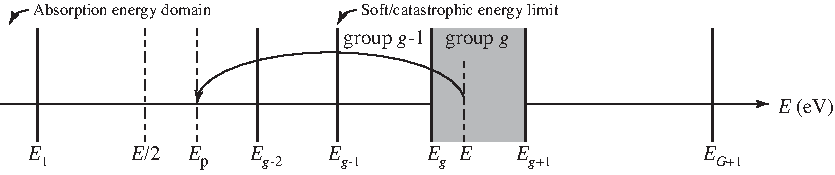
\includegraphics[keepaspectratio, width=5.0in, angle=0]{figs/electr1ack}
\caption[Description of the multigroup discretization] {Definition of the
arbitrary soft/catastrophic energy limit and of the absorption energy domain
below $E_1$.}
\label{electr-fig1}
\end{figure}

A catastrophic approximation of the collisional stopping power defined
in Eq.~\ref{elr_eq2} is also required. It is written
  \begin{equation}
     {\cal M}^{\rm col}_g(E)=\int_{E/2}^{E_{g-1}} dE_{\rm p} \,
     (E - E_{\rm p}) \, \sigma_{\rm col}(E\rightarrow E_{\rm p}) \, .
  \label{elr_eq3}
  \end{equation}

Unfortunately, it is not possible to compute ${\cal M}^{\rm col}_g(E)$ by
interpolating the collisional stopping power $s^{\rm col}(E)$ of
Eq.~\ref{elr_eq2} because the lower integration limit is not half the upper
limit in Eq.~\ref{elr_eq3}. As proposed in Ref.~\cite{CEPXS}, we use an
analytical expression of Eq.~\ref{elr_eq3}, obtained from the M\o{}ller
collision law as:
  \begin{equation}
    {\cal M}^{\rm col}_g(E) = {3Z\sigma_T \over 4\beta^2}\, E_0
    \left[ D_1 + {D_2 \over (k+1)^2} + D_3 \, {2k+1 \over (k+1)^2} \right]
  \label{elr_eq4}
  \end{equation}
\noindent with
\vspace{-0.6cm}
  \begin{eqnarray}
  D_1\negthinspace &=& \negthinspace
  2-{E\over E_{g-1}}+\ln\left[{E^2\over 4E_{g-1}\left(E-E_{g-1}\right)}
  \right] \\
  D_2\negthinspace &=& {1\over 2E_0^2}\left[E_{g-1}\left(2E-E_{g-1}\right)
  - {3E^2\over 4}\right] \\
  D_3\negthinspace &=& \negthinspace \ln\left({E\over 2E_{g-1}}\right)
  \end{eqnarray}
\noindent where
\begin{description}
\item [$Z$ =] atomic number of the atom
\item [$\sigma_T$ =] classical Thomson cross section (0.66524486 b)
\item [$E_0$ =] electron rest mass energy (511003.4 eV)
\item [$k$ =] energy of the incident electron in free-electron units ($k=E/E_0$)
\item [$\beta$ =] ratio of the electron velocity to the speed of light,
\end{description}
\noindent so that
  \begin{equation}
    \beta^2=1-{1\over(1+k)^2} \, .
  \end{equation}

\noindent This chapter describes ELECTR in version 2012.0.

\subsection{Description of Collision and Deposition Laws}
\label{ssELECTR_Desc}

There are two electrons coming out of each collision/ionization reaction with
an incident electron of energy $E$: the scattered electron and the recoil
electron. Because these two particles are identical, it is arbitrarily
assumed that the particle with the lower energy is the {\sl recoil electron},
and the one with the higher energy is the {\sl principal scattered electron}.
If $E_i$ is the binding energy for the sub-shell, the energy of the recoil
electron varies from 0 to $(E-E_i)/2$, and the energy of the scattered
electron varies from $(E-E_i)/2$ to $E-E_i$. Only the energy distribution
$P_{{\rm col},i}(E\rightarrow E_{\rm r})$ for the recoil electron is given
in File 26. The user can select a recoil energy $E_r$ from the distribution
and then generate the corresponding principal scattered electron with energy
$E-E_i-E_r$. It is assumed that no kinetic energy is transferred to the
residual atom.

This inelastic collision/electroionization reaction
\index{electroatomic!collision} is represented by the {\sl inelastic collision
law}\index{inelastic law} recovered from File 26. The value of $E_i$ is given
in the corresponding section of File 3 for each sub-shell.

The inelastic collision differential cross section for the principal and
recoil scattered electrons are represented by the formula:
  \begin{equation}
    \sigma_{\rm col}(E\rightarrow E',\mu)=\begin{cases}
    \sum_i\sigma_{{\rm col},i}(E) \,
    P_{{\rm col},i}(E\rightarrow E-E_i-E_{\rm p})\,
    \delta(\mu-\mu_{\rm p}) & \\ & \hspace{-7em}
    \text{if $E' \equiv E_{\rm p} \ge (E-E_i)/2$} \\
    \sum_i\sigma_{{\rm col},i}(E) \,
    P_{{\rm col},i}(E\rightarrow E_{\rm r}) \,
    \delta(\mu-\mu_{\rm r}) & \\ & \hspace{-7em}
    \text{if $E' \equiv E_{\rm r} < (E-E_i)/2$} \\
    \end{cases}
  \label{elr_eq5}
  \end{equation}
\noindent where
\begin{description}
\item [$E$ =] energy of the incident electron
\item [$i$ =] index of the ionized shell ($i=1$: $K$ shell; $i=2$: $L_1$
shell; $i=3$: $L_2$ shell; $i=4$: $L_3$ shell; $i=5$: $M$ shell, etc.).
Cross-section data for shells 1 to 39 are assigned to MT numbers 534$-$572.
\item [$E_i$ =] binding energy of shell $i$
\item [$E_{\rm r}$ =] energy of the recoil electron
\item [$E_{\rm p}$ =] energy of the principal scattered electron
($E_{\rm p}=E-E_i-E_{\rm p}$)
\item [$\mu$ =] scattering cosine
\item [$\sigma_{{\rm col},i}(E)$ =] microscopic cross section
\item [$P_{{\rm col},i}(E\rightarrow E_{\rm r})$ =] microscopic differential
energy distribution kernel for the recoil electron as recovered from File 26
\item [$\mu_{\rm p}$ =] deviation cosine of the principal scattered electron
\item [$\mu_{\rm r}$ =] deviation cosine of the recoil electron
\end{description}

\noindent The deviation cosine at which the principal scattered electron
emerges relative to the direction of the incident electron is given by the
following relation:
  \begin{equation}
    \mu_{\rm p} = \left[{E_{\rm p}(E-E_i+2E_0)\over (E-E_i)(E_{\rm p}+2E_0)}
    \right]^{1/2} \, .
  \label{elr_eq6}
  \end{equation}

\noindent The recoil electron emerges with a deviation cosine equal to
  \begin{equation}
    \mu_{\rm r} = \left[{E_{\rm r}(E-E_i+2E_0)\over (E-E_i)(E_{\rm r}+2E_0)}
    \right]^{1/2} \, .
  \label{elr_eq7}
  \end{equation}

The feed function for the restricted total inelastic cross section is
obtained by integrating Eq.~\ref{elr_eq5} over secondary energy of the
principal scattered electrons up to a threshold energy. We obtain
  \begin{equation}
     {\cal T}^{\rm col}_g(E)=\int_{E/2}^{E_{g-1}} dE_{\rm p} \,
     \sigma_{\rm col}(E\rightarrow E_{\rm p})
  \label{elr_eq8}
  \end{equation}
\noindent where the threshold energy limit is arbitrarily selected at the
interface $E_{g-1}$ between soft and catastrophic collisions.

The feed function ${\cal F}^{\rm col}$ represents the inelastic collision
contribution from $E$ into group $g'$. This feed function for is made of
two components, one corresponding to principal scattered electrons and one
corresponding to recoil electrons:
  \begin{eqnarray}
    \nonumber {\cal F}^{{\rm col},n}_{\ell g'}(E) \negthinspace
    &=& \negthinspace \int_{-1}^1 d\mu \,P_\ell(\mu) \int_{g'} dE'
    \, \sigma_{\rm col}(E\rightarrow E',\mu)\,(E')^n \\
    \nonumber &=& \negthinspace \int_{-1}^1 d\mu \, P_\ell(\mu)
    \bigg[ \int_{\max(E_{g'},E/2)}^{\min(E_{g'+1},E-E_{\rm cut})} dE' \,
    \sigma_{\rm col}(E\rightarrow E',\mu)\,(E')^n \\
    &~& + \,\int_{\max(E_{g'},E_{\rm cut})}^{\min(E_{g'+1},E/2)} dE' \,
    \sigma_{\rm col}(E\rightarrow E',\mu)\,(E')^n \bigg]
  \label{elr_eq9}
  \end{eqnarray}
\noindent where $E_{\rm cut}$ is a threshold integration limit chosen to avoid
the divergence of the feed function ${\cal F}^{{\rm col},n}_{\ell g'}(E)$ for
soft collisions. The feed function is computed for $0\le n\le 1$. It is
implicit in all integrals that the lower bound is smaller than the upper
bound.

Solution of the BFP equation requires the knowledge of the {\sl restricted
collisional stopping power} \index{electroatomic!stopping power} at specific
energy values $E$. The total collisional stopping powers (in units of MeV-barn)
$s^{\rm col}(E)$ are recovered from an ENDF evaluation (on unit {\tt nstop})
based on the Bethe theory and collected by Berger {\sl et al.}\cite{ICRU37}.
The catastrophic component of the collisional stopping powers are subtracted
from the total values to obtain the restricted collisional stopping powers
$r_g^{\rm col}(E)$ (corresponding to the soft component of stopping powers) as
  \begin{equation}
   r_g^{\rm col}(E) = s^{\rm col}(E) - {\cal M}^{\rm col}_g(E)
  \label{elr_eq10}
  \end{equation}
\noindent where $E_g < E \le E_{g+1}$. We observe that the soft collisions
in $s^{\rm col}(E)$ dominate collisional energy loss, even when an excessive
number of electron energy groups are used.

Energy-deposition cross sections are associated with every type of interaction.
These values are defined as the net energy deposited in the medium due to the
interactions of particles in a group in units of MeV-barn. The feed function
for the energy deposition cross sections ${\cal E}_g^{\rm col}(E)$ for the
inelastic interaction is the sum of catastrophic and soft components,
written as
  \begin{eqnarray}
  \nonumber {\cal E}_g^{\rm col,cata}(E)\negthinspace &=&\negthinspace 1\times
  10^{-6}\bigg[{\cal T}^{\rm col}_g(E)\, E -\sum_{h=1}^{g-2}
  {\cal F}^{{\rm col},1}_{0 h}(E)\bigg] \\
  {\cal E}_g^{\rm col,soft}(E)\negthinspace &=&\negthinspace 1\times
  10^{-6}\bigg[ s^{\rm col}(\bar E_g) - {\cal M}^{\rm col}_g(\bar E_g)\bigg]
  \label{elr_eq13}
  \end{eqnarray}
\noindent where $\bar E_g$ is the midpoint energy of electron group $g$.

The bremsstrahlung differential cross section
\index{electroatomic!bremsstrahlung} for the scattered electron and emitted
photon are represented by the following expressions:
  \begin{eqnarray}
    \nonumber \sigma_{\rm br}(E\rightarrow E',\mu) \negthinspace &=&
    \negthinspace\sigma_{\rm brp}(E\rightarrow E-E') \, \delta(\mu-1) \ \
    {\rm for \ the \ scattered \ electron} \\
    \sigma_{\rm brp}(E\rightarrow E_{\rm p},\mu) \negthinspace &=&
    \negthinspace\sigma_{\rm brp}(E\rightarrow E_{\rm p})
    \, D_{\rm br}(\mu_{\rm p}) \ \ {\rm for \ the \ emitted \ photon}
  \label{elr_eq14}
  \end{eqnarray}
\noindent where
\begin{description}
\item [$E$ =] energy of the incident electron
\item [$E'$ =] energy of the scattered electron
\item [$E_{\rm p}$ =] energy of the emitted photon ($E_{\rm p}=E-E'$). The
maximum energy of the emitted photon is arbitrarily assumed to be 1 keV
less than the energy of the incident electron.
\item [$\mu$ =] scattering cosine
\item [$\sigma_{\rm brp}(E\rightarrow E_{\rm p})$ =]
microscopic electron-photon bremsstrahlung differential cross section
kernel as recovered from File 26
\item [$\mu_{\rm p}$ =] deviation cosine of the emitted photon.
\end{description}

\noindent The deviation cosine at which the emitted photon emerges
relative to the direction of the incident electron is given by the
Sommerfield angular distribution\cite{SANDYL}:
  \begin{equation}
    D_{\rm br}(\mu_{\rm p}) = {1-\beta^2 \over 2\,(1-\beta \mu_{\rm p})^2} .
  \end{equation}

The feed function ${\cal F}^{\rm br}$ represents the bremsstrahlung
emission of secondary electrons into group $g'$. This function is written
  \begin{eqnarray}
    \nonumber {\cal F}^{{\rm br},n}_{\ell g'}(E) \negthinspace
    &=& \negthinspace \int_{-1}^1 d\mu \,P_\ell(\mu)\int_{g'} dE'
    \, \sigma_{\rm br}(E\rightarrow E',\mu)\,(E')^n \\
    &=& \negthinspace
    \int_{\max(E_{g'},E_{\rm min})}^{\min(E_{g'+1},E-E_{\rm cut})} dE' \,
    \sigma_{\rm brp}(E\rightarrow E-E')\,(E')^n
  \label{elr_eq15}
  \end{eqnarray}
\noindent where $E_{\rm min}$ is arbitrarily set to 1 keV.

The feed function ${\cal G}^{\rm br}$ represents the bremsstrahlung
emission of secondary photons into group $g'$. This function is written
  \begin{eqnarray}
    \nonumber {\cal G}^{{\rm br},n}_{\ell g'}(E) \negthinspace
    &=& \negthinspace \int_{-1}^1 d\mu_{\rm p} \,P_\ell(\mu_{\rm p})\int_{g'}
    dE' \, \sigma_{\rm brp}(E\rightarrow E',\mu_{\rm p})\,(E')^n \\
    \nonumber &=& \negthinspace \int_{-1}^1 d\mu_{\rm p} \,
    D_{\rm br}(\mu_{\rm p})\, P_\ell(\mu_{\rm p})
    \int_{\max(E_{g'},E_{\rm min})}^{\min(E_{g'+1},E-E_{\rm cut})}
    \negthinspace dE_{\rm p} \,\sigma_{\rm brp}(E\rightarrow E_{\rm p})\,
    (E')^n \, \, .\\
  \label{elr_eq16}
  \end{eqnarray}

Solution of the BFP equation requires the knowledge of the {\sl restricted
radiative stopping power} \index{electroatomic!stopping power} at specific
energy values $E$. The total radiative stopping powers (in units of MeV-barn)
$s^{\rm br}(E)$ are recovered from an evaluation by Berger
{\sl et al.}\cite{ICRU37}. The catastrophic component of the radiative
stopping powers are subtracted from the total values to obtain the
restricted radiative stopping powers $r_g^{\rm br}(E)$ as
  \begin{eqnarray}
   \nonumber r_g^{\rm br}(E) \negthinspace &=& \negthinspace s^{\rm br}(E) -
     \int_{E_{\rm min}}^{E_{g-1}} dE' \, (E-E')\,
     \sigma_{\rm br}(E\rightarrow E') \\
     &=& \negthinspace s^{\rm br}(E)-s^{\rm br}(E_{g-1})
  \label{elr_eq17}
  \end{eqnarray}
\noindent where $E_g < E \le E_{g+1}$. The magnitude of the stopping
power associated with catastrophic radiative loss is close to the total
radiative stopping power, even when few electron energy groups are used.

The feed function for the restricted total cross section
${\cal T}^{\rm br}_g(E)$ of a bremsstrah\-lung interaction is written
  \begin{equation}
  {\cal T}^{\rm br}_g(E)=\int_{E_{\rm min}}^{E_{g-1}} dE' \,
     \sigma_{\rm br}(E\rightarrow E')
  \label{elr_eq18}
  \end{equation}
\noindent where some contributions with $E'< E_{1}$ should be included.

The feed function for the energy deposition cross sections
${\cal E}_g^{\rm br}(E)$ for the secondary electron produced by a
bremsstrahlung interaction is the sum of catastrophic and soft components,
written as
  \begin{eqnarray}
  \nonumber {\cal E}_g^{\rm br,cata}(E)\negthinspace &=&\negthinspace 1\times
  10^{-6} \bigg[{\cal T}^{\rm br}_g(E)\, E  -\sum_{h=1}^{g-2}
  {\cal F}^{{\rm br},1}_{0 h}(E)\bigg] \\
  {\cal E}_g^{\rm br,soft}(E)\negthinspace &=&\negthinspace 1\times
  10^{-6}\bigg[ s^{\rm br}(\bar E_g) - s^{\rm br}(E_{g-1})\bigg]
  \label{elr_eq19}
  \end{eqnarray}
\noindent where $\bar E_g$ is the midpoint energy of electron group $g$.

The feed function for the energy deposition cross sections
${\cal E}_g^{\rm br}(E)$ for the secondary photon produced by a
bremsstrahlung interaction is written
  \begin{equation}
  {\cal E}_g^{{\rm br}\gamma}(E)=-1\times 10^{-6}\bigg[\sum_{h=1}^g
  {\cal G}^{{\rm br},1}_{0 h}(E)\bigg]
  \label{elr_eq20}
  \end{equation}
\noindent where $\bar E_g^\gamma$ is the midpoint energy of photon group $g$.

The Rutherford elastic collision cross section \index{electroatomic!Rutherford}
for the scattered electron is represented by the following expression:
  \begin{equation}
    \sigma_{\rm e}(E\rightarrow E',\mu) = \sigma_{\rm e}(E) \, \delta(E-E')
    \, D_{\rm e}(\mu)
  \label{elr_eq21}
  \end{equation}
\noindent where the scattered electron is deviated without change in energy
with a forward-peaked angular distribution $D_{\rm e}(\mu)$ recovered from
File 26. This highly forward-peaked elastic collision cross section is modified
by the {\sl extended transport correction}. This approximation makes the
elastic collision cross section compatible with a low-order Legendre expansion.

\noindent The within-group {\sl Rutherford feed function} ${\cal F}^{\rm e}$ is
the scattering contribution from $E$ into group $g$ containing $E$. The feed
function for elastic collision is written:
  \begin{equation}
    {\cal F}^{\rm e}_{\ell g}(E) = \int_{-1}^1 d\mu \int_{g} dE'
    \, \sigma_{\rm e}(E\rightarrow E',\mu)\,P_\ell(\mu) .
  \label{elr_eq22}
  \end{equation}

The transport-corrected within-group {\sl Rutherford feed function} is then
written as
  \begin{equation}
    \bar{\cal F}^{\rm e}_{\ell g}(E) = {\cal F}^{\rm e}_{\ell g}(E)-
    {\cal F}^{\rm e}_{L g}(E)
  \label{elr_eq23}
  \end{equation}
\noindent where $L$ is the maximum Legendre order.

A feed function for the charge deposition cross sections ${\cal C}_g(E)$
is associated to any electroatomic reaction with a non-zero absorption. A
positive value indicates electrons deposited while a negative value means
electrons are removed. The general definition of ${\cal C}_g(E)$ is written
  \begin{equation}
    {\cal C}_g(E) ={\cal T}_g(E)-\sum_{h=1}^{g-2} {\cal F}^0_{0 h}(E) \ .
  \label{elr_eq24}
  \end{equation}

\subsection{Atomic relaxation}
\label{ssELECTR_Relaxation}

Each atomic shell $i$ is characterized by a binding energy $E_i$.
Fig.~\ref{electr-fig5} represents the two atomic relaxation process available
in file 28 of the ENDF-102 specification. Atomic relaxation is a consequence
of a vacancy in an electronic shell following an electroatomic inelastic
collision or a photoatomic Klein-Nishina reaction. For example, if an incident
photon or electron of energy $E$ ionizes the $K$ shell with binding energy
$E_1$, the atom will emit an electron with energy $E - E_1$ , and the atomic
structure will be left ionized, with a vacancy in the $K$ shell.
\begin{itemize}
\item One way the atom can proceed to fill this hole is to bring down an
electron from a higher energy level, for example $L_1$, with the simultaneous
emission of an X-ray of energy $E_1 - E_2$. This is a radiative transition,
as depicted in Fig.~\ref{electr-fig5}.
\item An alternative path is to bring down an electron from a higher level
with the simultaneous emission of an electron from that level or a higher one.
As an example, you might see an electron of energy $E_1 -E_2 -E_3$,
which fills the vacancy in the $K$ shell and leaves new holes in the $L_1$ and
$L_2$ shells. These are called Auger transitions, also depicted in
Fig.~\ref{electr-fig5}.
\end{itemize}

\begin{figure}[h!]
\centering
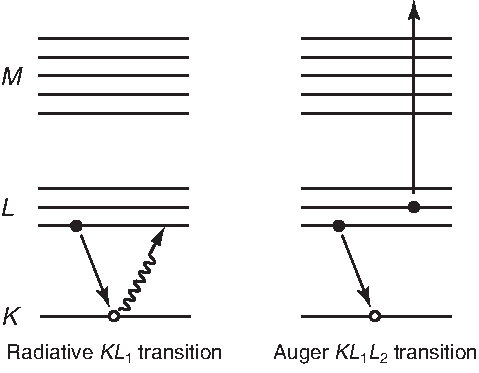
\includegraphics[keepaspectratio, width=2.5in, angle=0]{figs/electr_relaxation}
\caption[Radiative and Auger atomic relaxation] {Definition of the
$KL$ and $KLL$ notations for atomic relaxation.}
\label{electr-fig5}
\end{figure}

The radiative transitions are denoted by labels of the form $WX$ where $W$ is
the shell in which the original vacancy occurs and $X$ is the shell from which
the $W$ vacancy is filled with an emission of a photon representing the energy
between shells $W$ and $X$. Similarly, the Auger transitions are denoted by
labels of the form $WXY$, where $W$ is the shell in which the original vacancy
occurs, $X$ is the shell from which the $W$ vacancy is filled, and $Y$ is the
shell from which the Auger electron is ejected

The {\sl impact electroionization feed function} ${\cal F}_i^{\rm I}$
\index{electroatomic!impact} for the Auger electron is represented by
the following expression:
  \begin{equation}
    {\cal F}^{\rm I}_{i,\ell g}(E) =  \begin{cases}
    \sigma^{\rm I}_i(E) \sum_{j=1}^{N_{\rm tr}}
    \eta_{i,j}^{\rm e} \, \delta_{g,g_j} & \text{if $\ell=0$} \\
    0 & \text{if $\ell>0$} \end{cases}
  \label{elr_eq25}
  \end{equation}
\noindent where
\begin{description}
\item [$E$ =] energy of the incident electron
\item [$N_{\rm tr}$ =] number of transitions
\item [$i$ =] index of the ionized shell ($i=1$: $K$ shell; $i=2$: $L_1$
shell; $i=3$: $L_2$ shell; $i=4$: $L_3$ shell; $i=5$: $M$ shell, etc.).
Cross-section data for shells 1 to 39 are assigned to MT numbers 534$-$572.
\item [$j$ =] index of the transition radiation
\item [$\eta_{i,j}^{\rm e}$ =] relaxation efficiency that the $j^{\rm th}$
transition produces Auger electrons following the ionization of the
$i^{\rm th}$ shell
\item [$g_j$ =] electron group that contains the energy of the
$j^{\rm th}$ Auger electron.
\end{description}

The corresponding feed function for the energy deposition cross sections
${\cal E}_i^{\rm I}(E)$ caused by Auger electrons is written
  \begin{equation}
    {\cal E}^{\rm I}_{i,g}(E) =
    -\sigma^{\rm I}_i(E) \sum_{j=1}^{N_{\rm tr}} \eta_{i,j}^{\rm e} \,
    e_{i,j}^{\rm e} \,\delta_{g,g_j}
  \label{elr_eq26}
  \end{equation}
\noindent where $e_{i,j}^{\rm e}$ is the energy of the Auger electron.

The {impact electroionization feed function} ${\cal G}^{\rm I}_i$
\index{electroatomic!impact} for fluorescence production is represented by
the following expression:
  \begin{equation}
    {\cal G}^{\rm I}_{i,\ell,f}(E) =  \begin{cases}
    \sigma^{\rm I}_i(E) \sum_{j=1}^{N_{\rm tr}} \eta_{i,j}^{\rm f} \,
    \delta_{f,f_j} & \text{if $\ell=0$} \\
    0 & \text{if $\ell>0$} \end{cases}
  \label{elr_eq27}
  \end{equation}
\begin{description}
\item [$\eta_{i,j}^{\rm f}$ =] relaxation efficiency that the $j^{\rm th}$
transition produces fluorescence photons following the ionization of the
$i^{\rm th}$ shell
\item [$f_j$ =] photon group that contains the energy of the
$j^{\rm th}$ fluorescence photon.
\end{description}

The corresponding feed function for the energy deposition cross sections
${\cal E}_i^{{\rm I}\gamma}(E)$ caused by fluorescence photons is written
  \begin{equation}
    {\cal E}^{{\rm I}\gamma}_{i,f}(E) =
    -\sigma^{\rm I}_i(E) \sum_{j=1}^{N_{\rm tr}} \eta_{i,j}^{\rm f} \,
    e_{i,j}^{\rm f} \,\delta_{f,f_j}
  \label{elr_eq28}
  \end{equation}
\noindent where $e_{i,j}^{\rm f}$ is the energy of the emitted photon.

\subsection{Calculational Method}
\label{ssELECTR_CalcMethod}

Multigroup cross sections are obtained by Lobatto quadrature of the feed
function assigned to each electroatomic reaction. Vector and matrix cross
sections data structures are defined as

  \begin{eqnarray}
    \sigma_{xg}&=&{{\int_g{\cal F}^x(E)\,\phi_0(E)\,dE}
    \over {\int_g\phi_0(E)\,dE}} \ \ ,
    \mbox{}\\
    \sigma_{x\ell g\rightarrow g'}&=&
    {{\int_g{\cal F}^x_{\ell g'}(E)\,\phi_\ell(E)\,dE}
    \over {\int_g\phi_\ell(E)\,dE}} \ \ \hbox{and}\\
    \sigma_{x\ell g\rightarrow g'}^\gamma&=&
    {{\int_g{\cal G}^x_{\ell g'}(E)\,\phi_\ell(E)\,dE}
    \over {\int_g\phi_\ell(E)\,dE}} \,\,.
  \label{elr_eq29}
  \end{eqnarray}

\noindent
In these expressions, $g$ represents an energy group for the initial
energy $E$, $g'$ is a group of final energies $E'$, $x$ stands for one
of the reaction types and $\phi_\ell$ is a Legendre component of a
guess for the electron flux. The electroatomic cross sections
$\sigma_x(E)$ are already included in the feed function
${\cal F}^x_{\ell g'}(E)$ of Eqs.~\ref{elr_eq9}, \ref{elr_eq15},
\ref{elr_eq23} and~\ref{elr_eq24}. Similarly, electroatomic cross sections
$\sigma_x^\gamma(E)$ are already included in the feed function
${\cal G}^x_{\ell g'}(E)$ of Eqs.~\ref{elr_eq16} and~\ref{elr_eq27}.

For reaction types corresponding to inelastic and bremsstrahlung, the
{\sl catastrophic} components $\sigma_{x\ell g\rightarrow g'}$ of the
scattering differential cross sections are arbitrarily defined for principal
scattered electron energies corresponding to groups $g'\le g-2$, where
$E_g < E\le E_{g+1}$.

\subsection{Cross sections for the restricted CSD operator}
\label{ssELECTR_CSDOperator}

The restricted collision {\sl and} radiative stopping power must be
evaluated at all electron group boundaries. These values are required
in the second-order difference form of the {\sl continuous slowing
down} (CSD) operator. The restricted stopping power at boundary energy
$E_g$ with $1 \le g \le G+1$ is the average of the value at the
upper boundary of group $g-1$ and the value at the lower boundary of
group $g$:
  \begin{equation}
    r_g^{\rm CSD} = \begin{cases}
    {1\over 2}\left[ r_{g-1}(E_g)+ r_g(E_g)\right] & \text{if $g>1$} \\
    {1\over 2}\, r_{1}(E_1) & \text{if $g=1$} \end{cases}
  \label{elr_eq30}
  \end{equation}
\noindent where $r_g(E)$ is given by Eqs.~(\ref{elr_eq10})
and~(\ref{elr_eq30}).

\subsection{Coding Details}
\label{ssELECTR_details}

The main entry point is subroutine \cword{electr} exported by
module \cword{electm}\index{modules!electm@{\ty electm}}.
The code begins by reading the user's input. It then locates the
position for the new material on the old GENDF\index{GENDF}
tape (if any) and copies the earlier results to the new output
tape. The desired material is also located on the input
PENDF\index{PENDF} tape prepared previously using
\hyperlink{sRECONRhy}{RECONR}\index{RECONR}.
A new material header is then written onto the output tape leaving
the code ready to begin the loop over reaction types.

For each of the preset reaction types, ELECTR uses the panel logic
of \hyperlink{sGROUPRhy}{GROUPR}\index{GROUPR} to average the cross
sections (see the ``panel" discussion in Section~\ref{ssGROUPR_GrpInt}).
The resulting cross sections and group-to-group matrix elements are
then printed out and written to the output tape. The restricted total
cross section and the energy and charge deposition contributions from
each reaction are summed into a storage area. After all reactions have
been processed for this material, a special pass through the output
logic is used to create the restricted total cross section in MT=501
and the energy and charge deposition cross section in MT=530 and MT=531.
Finally, the rest of the old output tape is copied to the new output
tape. A description of the format of the multigroup output tape will
be found in the \hyperlink{sGROUPRhy}{GROUPR} chapter (see
Section~\ref{ssGROUPR_GENDF}).

As with \cword{panel} in \hyperlink{sGROUPRhy}{GROUPR},
\cword{epanel}\index{epanel@{\ty epanel}} integrates the triple product
${\cal F}{*}\sigma{*}\phi$.  The feed into secondary group $g'$ for
Legendre order $\ell$ from initial energy $E$ is computed in
\cword{etff}\index{etff@{\ty etff}}. Cross sections are read from
the PENDF tape (see \cword{gtsig}\index{gtsig@{\ty gtsig}}). Flux can
be read in, constant, or $1/E$ with high and low energy roll-offs (see
\cword{enwtf}\index{enwtf@{\ty enwtf}} and
\cword{etflx}\index{etflx@{\ty etflx}}).

Scattering laws of type {\tt LAW} $=1$ for collision/ionization inelastic
and bremss\-trahlung reactions are stored in {\tt TAB2} records similar to
those used for neutron-induced reactions in \hyperlink{sGROUPRhy}{GROUPR}
\index{GROUPR} where {\tt tab1io} data structures are replaced by {\tt listio}
data structures. The subroutine \cword{eetsed}\index{eetsed@{\ty eetsed}}
returns the secondary-energy distribution for electrons for all groups
simultaneously, using an implementation similar to subroutines \cword{getsed}
of \index{getsed@{\ty getsed}} GROUPR.

The subroutine \cword{eetsed} is initialized for a particular reaction by
calling it with \cword{ed} $=0$. First, scratch storage is allocated, and
all the subsections are read in. Tabulated subsections are averaged over
outgoing energy groups for each of the given incident energies.  The array
\cword{loc} contains pointers for each subsection. On subsequent entries
(\cword{ed}$>$0), \cword{eetsed} loops over the subsections for this reaction.
It first retrieves the fractional probability for the subsection using
\cword{terpa}\index{terpa@{\ty terpa}}. The routine interpolates between
values of the tabulated data using the {\sl unit base interpolation
technique}, multiply by the fractional probability for the law and
accumulates the contributions into \cword{sed}. ENDF TAB2 information
available in MF=26 is only related to recoil electrons or emitted photon
probability law $P(E\rightarrow E_{\rm r})$. Additional subsections are
generated by \cword{eetsed} with \cword{ed} $=0$ to enable the processing
of probability law for the principal scattered electron and for the first
moments $P(E\rightarrow E_{\rm r})E_{\rm r}$ of these probability laws.

\subsection{User Input}
\label{ssELECTR_UserInp}

The following description of the user input is reproduced from
the comment cards at the beginning of the ELECTR module.
\index{ELECTR!ELECTR input}
\index{input!ELECTR}

\small
\begin{ccode}

   !---input specifications (free format)---------------------------
   !
   ! card1
   !    nendf   unit for endf tape
   !    npend   unit for pendf tape
   !    nstop   unit for output stopping power tape in endf-102 format
   !    nacti   unit for atomic relaxation tape
   !    nbet1   unit for input nbet tape (default=0)
   !    nbet2   unit for output nbet tape (default=0)
   ! card2
   !    matb    material to be processed
   !            input materials in ascending order
   !    ige     electron group structure option
   !    igg     gamma group structure option (=0 for single set)
   !    iwt     weight function option
   !    lord    Legendre order
   !    iprint  print option (0/1=minimum/maximum) (default=1)
   ! card3
   !    title   run label up to 80 characters (delimited by ',
   !            ended with /)
   ! card4      (ige=-2 or -1 only)
   !    nge     number of electron groups
   !    emin    minimum energy bound (ev)
   !    emax    maximum energy bound (ev)
   ! card4      (ige=1 only)
   !    nge     number of electron groups
   !    ege     nge+1 group bounds (ev)
   ! card5      (igg=-2 or -1 only)
   !    ngg     number of photon groups
   !    gmin    minimum energy bound (ev)
   !    gmax    maximum energy bound (ev)
   ! card5      (igg=1 only)
   !    ngg     number of photon groups
   !    egg     ngg+1 group bounds (ev)
   ! card6      (iwt=1 only)
   !    wght    weight function as tab1 record
   ! card7
   !    mfd     file to be processed
   !    mtd     section to be processed
   !    mtname  description of section to be processed
   !            repeat for all reactions desired
   !            mfd=0/ terminates this material
   !            mfd=-1/ is a flag to process all sections present
   !            for this material  (termination is automatic)
   ! card8
   !    matd    next mat number to be processed
   !            terminate electr run with matd=0.
   !
   !---options for input variables----------------------------------
   !
   !        ige     meaning
   !        ---     -------
   !        -2      uniform logarithmic group structure
   !        -1      uniform linear group structure
   !         0      none
   !         1      arbitrary structure (read in)
   !         2      csewg 94-group structure
   !         3      lanl 12-group structure
   !         4      steiner 21-group gamma-ray structure
   !         5      straker 22-group structure
   !         6      lanl 48-group structure
   !         7      lanl 24-group structure
   !         8      vitamin-c 36-group structure
   !         9      vitamin-e 38-group structure
   !         10     vitamin-j 42-group structure
   !
   !        iwt     meaning
   !        ---     -------
   !         1      read in
   !         2      constant
   !         3      1/e + rolloffs
   !
   !------------------------------------------------------------------

\end{ccode}
\normalsize

Material numbers (\cword{matb}) are simply the element $Z$ number
for ENDF versions IV and V;  they are equal to $100{*}Z$ for
ENDF-6 formatted files. The normal mode of operation uses
\cword{mfd}$=-1$ for automatic processing of available MT reactions.

The following sample run prepares a MATXS tape for tungsten.
The numbers on the left are for reference; they are not part of the input.

\small
\begin{ccode}

  1.   reconr
  2.   30 31
  3.   'pendf tape for electron interaction cross sections from EPICS2017'/
  4.   7400 1 0
  5.   .001/
  6.   '1-tugnsten'/
  7.   0/
  8.   electr
  9.   30 31 38 39 0 33
 10.   7400 3 3 2 7 1
 11.   '12 group electron interaction library'/
 12.   -1 0/
 13.   0/
 14.   matxsr
 15.   0  0 35  0  0  0  0  0  0 33/
 16.   1 't2lanl njoy'/
 17.   2 2 1 1
 18.   '12-group electron interaction library'/
 19.   'b' 'g'/
 20.   12 12
 21.   'bscat' 'bgamma'/
 22.   1 1
 23.   1 2
 24.   'w' 7400 7400
 25.   stop

\end{ccode}
\normalsize

On line 2, an ENDF/B tape containing File 23 has been
mounted on logical unit 30. The title on line 3 will appear on the PENDF
tape. Material 7400 is tugnsten. The element name on line 6 will
appear on the PENDF tape in MF=1,MT=451. The linearization is accurate to
better than 0.1\%.  A more complete description of
\hyperlink{sRECONRhy}{RECONR's} input may be found in
Section~\ref{ssRECONR_inp}.

ELECTR uses the same ENDF tape as \hyperlink{sRECONRhy}{RECONR}
(actually only MF=26 is read by ELECTR), but ELECTR also reads the
\hyperlink{sRECONRhy}{RECONR} output tape on unit 31, the ENDF/B stopping
power tape on unit 38 and the ENDF atomic relaxation tape on unit 39.
The ELECTR GENDF tape will be on unit 33. Card 13 specifies tugnsten
as the material, 12 groups, constant weight, Legendre components
through P$_6$, and the full printed output. Line 25 terminates
the element loop and the ELECTR run.

Starting with ENDF/B-VI, the electron interaction (or electroatomic)
files contain detailed electroatomic cross sections, not just
the MT=522 total electroatomic cross section.  These electroatomic
cross sections have MT numbers starting with 534. ELECTR input is
somewhat more complicated when these reactions are included because
they are different for every element.

\subsection{Error Messages}

\begin{description}
\begin{singlespace}

\item[\cword{error in eenggp***illegal group structure}] ~\par
  Values of \cword{IGG} must lie between -2 and 10.

\item[\cword{error in eenggp***too many groups.}] ~\par
  Increase the size of the global array \cword{egg} by changing the
  parameter \cword{ngmax}=400 located at the start of the module.

\item[\cword{error in enwtf***illegal iwt}] ~\par
  Values of \cword{iwt} must lie between 1 and 3.

\item[\cword{error in epanel***elo gt ehi.}] ~\par
  There is something wrong with the energy grids during integration
  over incident energy. This usually means there is a problem with
  the choice of \cword{rndoff} and/or \cword{delta}.  Be sure that
  \cword{rndoff}$<$1, \cword{delta}$>$1, and \cword{rndoff*delta}$<$1
  as represented on your machine.

\item[\cword{error in etff***illegal file type.}] ~\par
  Only files 23 and 26 can be requested.

\item[\cword{error in etff***illegal reaction for cross section=---}] ~\par
  Only reactions 525, 527, 534 to 572, 507, 508, 501, 530 and 531 can
  be requested.

\end{singlespace}
\end{description}

\subsection{I/O Units}
\label{ssELECTR_IO}

There are no scratch files used in ELECTR. The only restriction
on the files assigned on line 1 of the user input is that \cword{nbet1} and
\cword{nbet2} must be in the same mode (that is, both binary or both
formatted).

\cleardoublepage
